\documentclass[11pt,a4paper]{article}
\usepackage[margin=23mm]{geometry}
\usepackage{amsmath,amssymb,booktabs,xcolor,graphicx,hyperref,siunitx}
\usepackage{fancyhdr}
\definecolor{navy}{HTML}{142D40}\definecolor{teal}{HTML}{087F82}
\hypersetup{colorlinks=true,linkcolor=teal,urlcolor=teal}
\pagestyle{fancy}\fancyhf{}\lhead{\small JU Mechanical Engineering}\rhead{\small Major Project 4.1 / 4.2}\cfoot{\thepage}
\setlength{\parindent}{0pt}\setlength{\parskip}{5pt}
\newcommand{\sect}[1]{\section*{\textcolor{teal}{#1}}}
\begin{document}
{\LARGE\bfseries\color{navy} Mathematical analysis and design audit}\par
{\large Modified Solar-Assisted Hollow-Cylinder Paddy Dryer}\par
Parth Pariwandh \quad Supervisor: Prof. Dulal Krishna Mandal\\
27 November 2026 \quad Preliminary review v1.0 (not experimental results)
\sect{1. Input basis and dimensional conventions}
The integrated 9 October and progress 29 October notes establish the reference 100 kg scale. The 80\,\si{\celsius} inlet and six-hour window are alternate assumed conditions, not approved or demonstrated. Initial trials are proposed at 40--45\,\si{\celsius}, with supervisor-approved grain limits.
\begin{center}\begin{tabular}{ll@{\qquad}ll}\toprule
Quantity&Assumption&Quantity&Assumption\\\midrule
$m_i$&100 kg&$\rho_b$&560 kg/m$^3$\\
$M_i,M_f$&0.22, 0.14&$L$&0.600 m\\
$D,d$&0.670, 0.250 m&$t,t_i$&0.002, 0.0012 m\\
$P$&101.325 kPa&$\tau$&21600 s\\
$T_a,\phi_a$&30\,\si{\celsius}, 0.70&$T_o,\phi_o$&45\,\si{\celsius}, 0.70\\
$T_{in}$&80\,\si{\celsius} (alternate)&$\epsilon,d_p$&0.45, 0.0025 m\\
$\mu$&$2.07\times10^{-5}$ Pa s&$\alpha,G$&0.90, 600 W/m$^2$\\
$h_{fg},c_{p,g}$&2406 kJ/kg, 1.7 kJ/(kg K)&$\Delta T_g$&15 K\\\bottomrule
\end{tabular}\end{center}
\sect{2. Conservation of dry matter}
Wet-basis moisture $M=m_w/(m_w+m_d)$, dry-basis moisture $X=m_w/m_d=M/(1-M)$; both are dimensionless mass ratios. With no loss of grain or solids, $m_d$ is conserved:
\begin{align}
m_d&=m_i(1-M_i)=100(0.78)=78\ \mathrm{kg},\\
m_f&=\frac{m_d}{1-M_f}=\frac{78}{0.86}=90.6977\ \mathrm{kg},\\
m_{ev}&=m_i-m_f=m_i\frac{M_i-M_f}{1-M_f}=9.3023\ \mathrm{kg}.
\end{align}
The final water content is $m_f-m_d=12.6977$ kg. The removal is not simply eight kilograms because the final wet mass is smaller. Dry-basis moisture decreases from $0.28205$ to $0.16279$ kg water/kg dry solids.\par
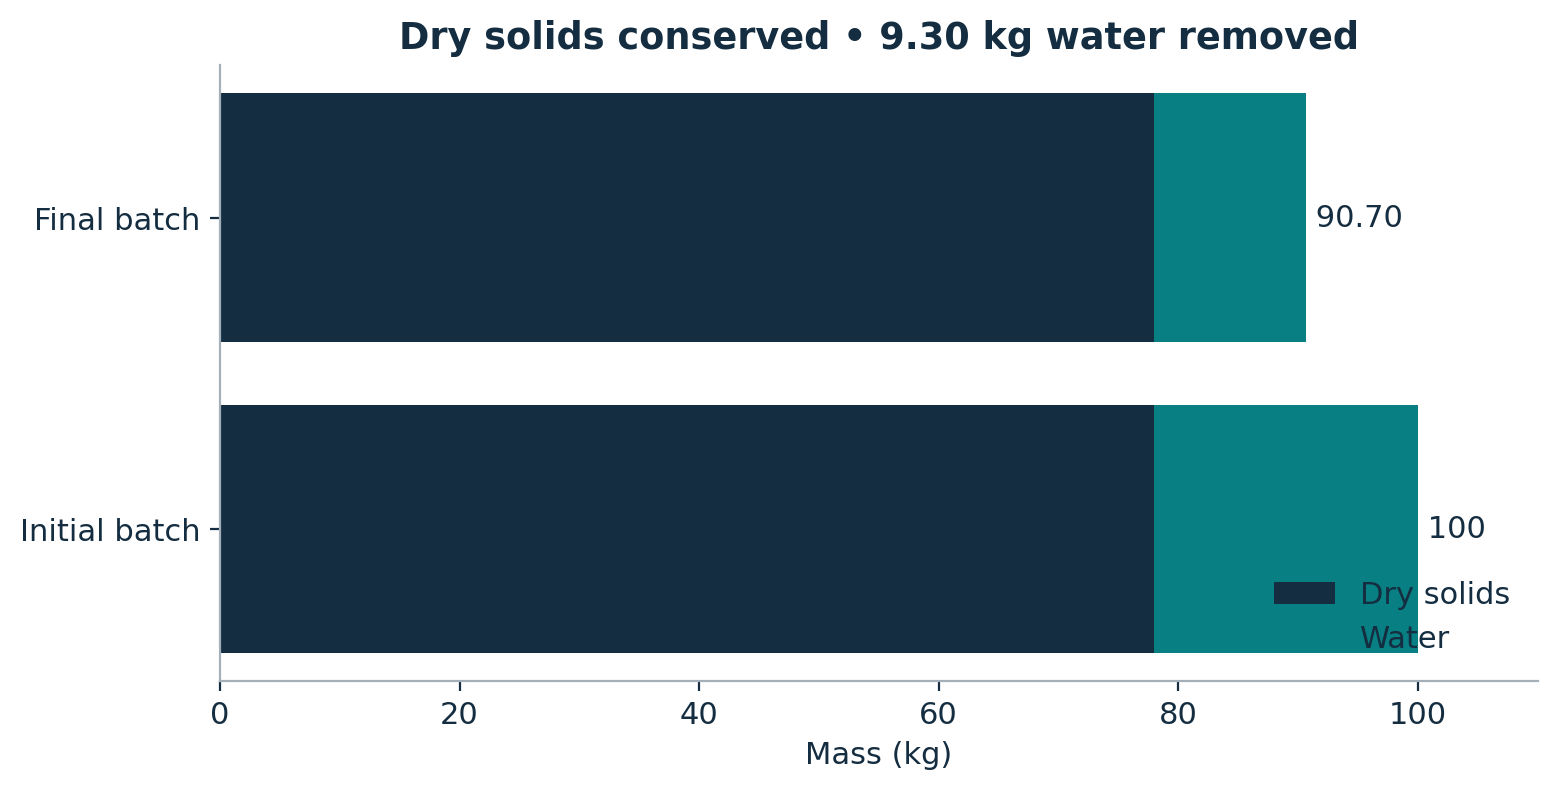
\includegraphics[width=.84\linewidth]{../figures/mass_balance.png}
\newpage
\sect{3. Annular geometry}
With $R=(D-2t)/2$ the inner radius of the outer wall and $r=d/2$ the outer radius of the core shell,
\begin{align}
V_{req}&=m_i/\rho_b=100/560=0.178571\ \mathrm{m^3},\\
A_{req}&=V_{req}/L=0.297619\ \mathrm{m^2},\\
D_{req}&=2\sqrt{A_{req}/\pi+r^2}+2t=0.668410\ \mathrm{m}.
\end{align}
Exact rounded model: $D=0.670$ m, $r=0.125$ m, $R=0.333$ m; $A=\pi(R^2-r^2)=0.299281$ m$^2$, $V=AL=0.179568$ m$^3$, $m_{cap}=\rho_bV=100.5583$ kg. Radial gap $R-r=0.208$ m. The small capacity mismatch is rounding; the actual density is unmeasured. Shell model assumes height equals fill, with freeboard and structure left for later design.\par
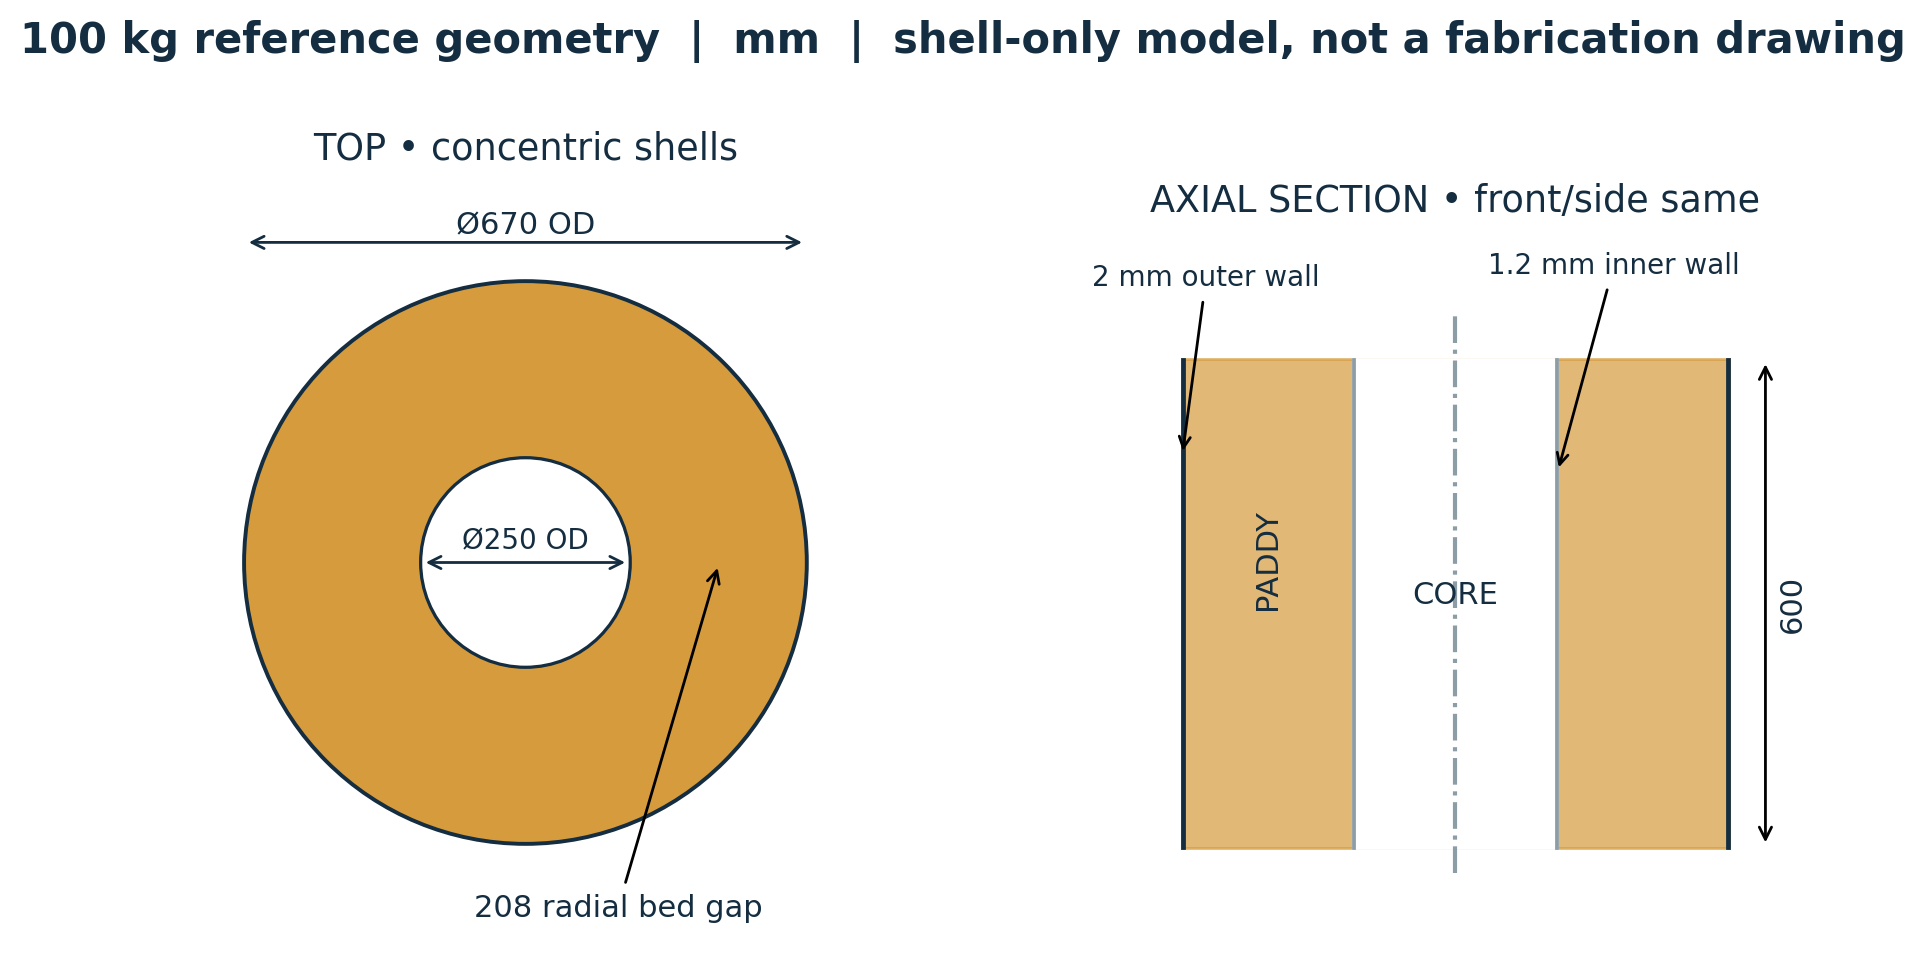
\includegraphics[width=\linewidth]{../figures/dimensioned_views.png}
\sect{4. Heat transfer through a thin wall}
For steady one-dimensional radial conduction with constant conductivity $k_s$ (W/m K), Fourier's law $q=-k_s A\,dT/dr$ yields
\begin{align}
R_{th}&=\frac{\ln(r_o/r_i)}{2\pi k_sL}\quad[\mathrm{K/W}],&\dot Q_{cond}&=\frac{T_o-T_i}{R_{th}}.
\end{align}
At $r_o=0.335$, $r_i=0.333$ m, $k_s=45$ W/(m K) (illustrative steel), $R_{th}=3.53\times10^{-5}$ K/W. A hypothetical 5 K wall drop would imply about 142 kW, not physically available solar power. At 217 W the drop is only 0.008 K. Heat available is limited by absorption and transfer/losses. Convection: $\dot Q=h_c A_s(T_s-T_a)$ with $h_c$ W/(m$^2$ K); radiation: $\dot Q_{rad}=\epsilon_s\sigma A_s(T_s^4-T_{sur}^4)$, absolute temperatures in kelvin, $\sigma=5.67\times10^{-8}$ W/(m$^2$ K$^4$). For $\epsilon_s=0.9$ and 45 vs 30\,\si{\celsius}, radiation is about 92 W/m$^2$; sky conditions can change this.
\newpage
\sect{5. Humidity and air mass flow}
For atmospheric moist air (ideal mixture), water-vapour partial pressure $p_v=\phi p_{sat}(T)$, RH $\phi$ as a fraction, and humidity ratio $\omega$ in kg water/kg dry air:
\begin{equation}
\omega=0.622\frac{p_v}{P-p_v},\quad p_{sat}\simeq0.61094\exp\!\left(\frac{17.625T}{T+243.04}\right)\ \mathrm{kPa}.
\end{equation}
$T$ is Celsius in this approximate saturation expression, which is a screening correlation (use accurate steam/psychrometric tables for final sizing). The model gives $\omega_i=0.018754$, $\omega_o=0.044135$, $\Delta\omega=0.025381$. Sensible heating leaves $\omega_i$ unchanged; at 43\,\si{\celsius} RH $\approx34.3\%$, at 80\,\si{\celsius} roughly 6\%.
\begin{align}
\dot m_{ev}&=9.3023/21600=4.3066\times10^{-4}\ \mathrm{kg/s},\\
\dot m_{da}&=\dot m_{ev}/(\omega_o-\omega_i)=0.016968\ \mathrm{kg/s},\\
v_{da}&=\frac{0.287042(T+273.15)(1+1.607858\omega_i)}{P}=1.03060\ \mathrm{m^3/kg_{da}},\\
\dot V&=\dot m_{da}v_{da}=0.017487\ \mathrm{m^3/s}=62.95\ \mathrm{m^3/h},\\
u&=\dot V/A=0.05843\ \mathrm{m/s}.
\end{align}
Assumptions: no leakage, dry-air steady flow, nominal average pickup and drying time. The original 61 m$^3$/h used approximate density. The refined number is conditional and not evidence of six-hour performance. For a 75 mm duct, mean speed is $\dot V/(\pi D_{duct}^2/4)\approx3.96$ m/s.
\sect{6. Useful heat and solar scale}
\begin{align}
Q_{ev}&=m_{ev}h_{fg}=22.381\ \mathrm{MJ},\\
Q_g&=m_i c_{p,g}\Delta T_g=2.550\ \mathrm{MJ},\\
Q_u&=24.931\ \mathrm{MJ},\\
\dot Q_{legacy}&=1.5Q_u/\tau=1.731\ \mathrm{kW},\\
\dot Q_{solar,gross}&=\alpha GDL=0.9(600)(0.670)(0.600)=217.08\ \mathrm W.
\end{align}
The 50\% additive allowance is not a measured efficiency. Gross solar input would be 4.69 MJ over six hours only if the assumed irradiation persisted and the projected area were valid. Real solar gain depends on beam angle, sky diffuse contribution, convective and radiative loss. It is not guaranteed heater capacity. The nominal useful average heat is 1.154 kW, showing why the small absorber is supplementary.
\newpage
\sect{7. Control-volume energy audit}
Moist-air enthalpy relative to 0\,\si{\celsius} liquid water:
\[h(T,\omega)=1.006T+\omega(2501+1.86T)\quad[\mathrm{kJ/kg_{da}}].\]
The assumed ambient, alternate inlet and exhaust states give respectively 78.13, 130.17 and 159.35 kJ/kg dry air. The heater upstream of the bed, ignoring its losses, requires
\[\dot Q_{pre}=\dot m_{da}(h_{in}-h_a)=0.883\ \mathrm{kW}.\]
For a transient bed with dry matter and retained liquid included in its stored energy $U_b$, neglecting kinetic/potential energy and shaft work:
\[\dot Q_{bed,net}=\dot m_{da}(h_o-h_{in})+\frac{dU_b}{dt}.\]
Here net heat includes solar through wall and any other heat entering bed minus losses; $U_b$ includes energy of liquid water being removed, so its time derivative accounts for the changing liquid inventory. $\dot m_{da}(h_o-h_{in})=0.495$ kW. The decreasing liquid inventory at about 30--45\,\si{\celsius} contributes roughly $-0.054$ to $-0.081$ kW at the nominal removal rate, whereas warming grain adds energy storage. Gross 0.217 kW solar cannot by itself supply the implied bed enthalpy rise under the assumed states and ordinary warming. A complete transient balance must measure grain/air states and losses. Do not add a separate latent term again to the enthalpy increase. Do not certify the 2.5 kW heater using these inconsistent legacy assumptions.\par
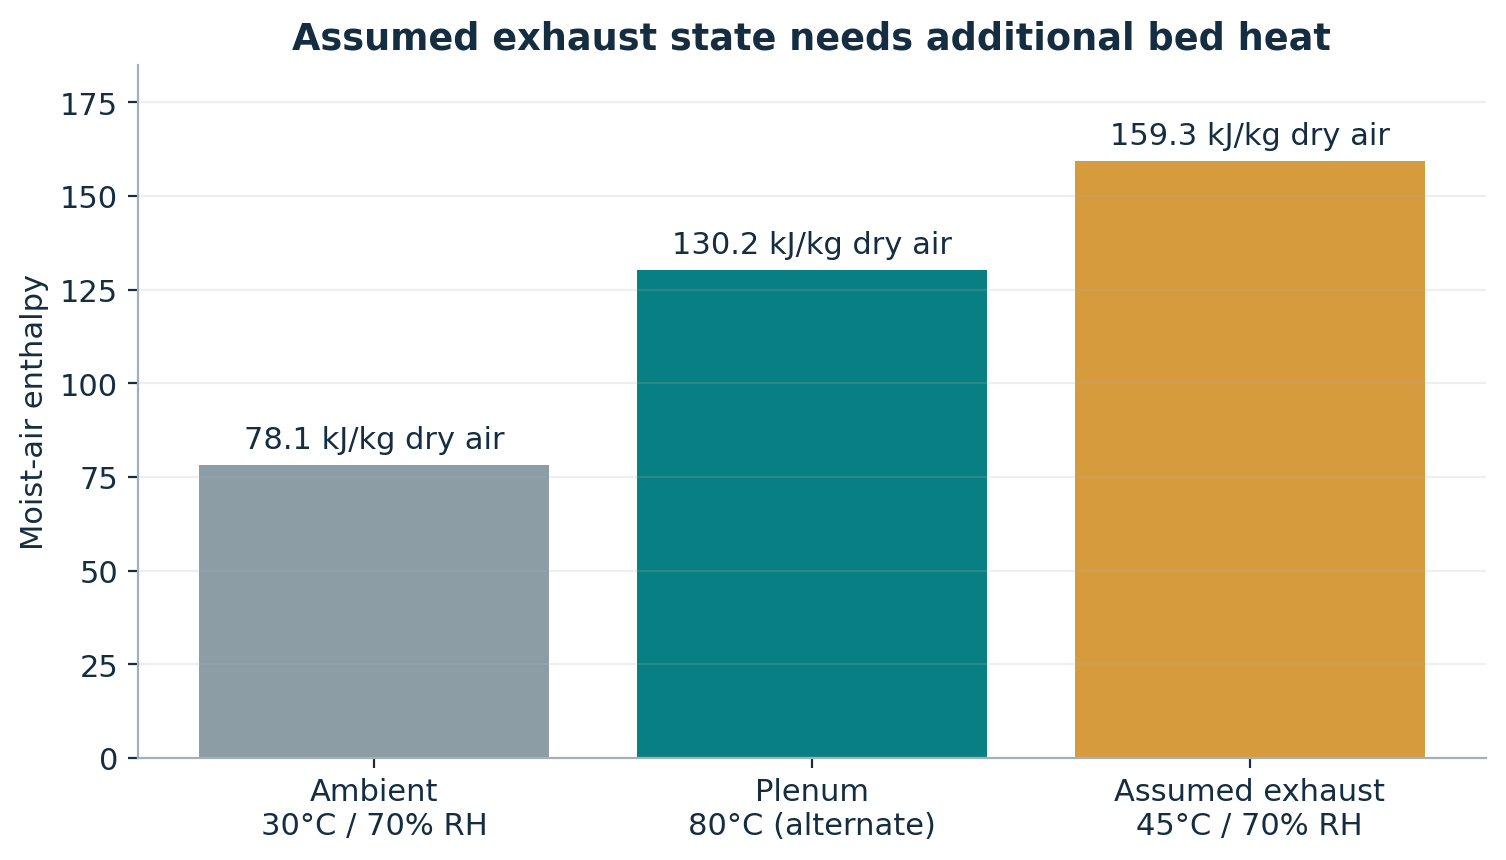
\includegraphics[width=.66\linewidth]{../figures/enthalpy.png}
\sect{8. Air resistance and open area}
Ergun screening correlation for packed beds, $u$ superficial velocity, $d_p$ equivalent particle diameter, $\rho_a$ moist-air density, $\mu$ viscosity, $\epsilon$ voidage:
\[\frac{\Delta P}{L}=\frac{150\mu(1-\epsilon)^2u}{\epsilon^3d_p^2}+\frac{1.75\rho_a(1-\epsilon)u^2}{\epsilon^3d_p}.\]
At the legacy values ($u=0.057$ m/s, $\rho_a=1$ kg/m$^3$), $\Delta P=64.64$ Pa. Refined flow and density $\rho_a=(1+\omega_i)/v_{da}$ give about 66.4 Pa. Bed air power $\dot V\Delta P=1.16$ W, shaft power $\dot V\Delta P/\eta_f=2.58$ W at $\eta_f=0.45$. Measure total resistance; select a real fan curve. The hole area per triangular unit cell is $\beta=\pi d_h^2/(2\sqrt3 p_h^2)$, dimensionless. Inner holes 1.5/6 mm: 5.668\%; upper outer vents 2/12 mm: 2.519\% locally. Test grain retention and clogging.
\newpage
\sect{9. Drying kinetics and validation}
Use local equilibrium moisture $X_e=f(T,\phi)$ from a suitable paddy sorption relation, not an invented constant. A first-order falling-rate model gives
\[\frac{dX}{dt}=-k(X-X_e)\quad\Rightarrow\quad MR=\frac{X-X_e}{X_0-X_e}=e^{-kt}.\]
This assumes constant $X_e$ and $k$ (s$^{-1}$). The empirical Page form $MR=e^{-kt^n}$ uses $k$ in s$^{-n}$ and dimensionless $n$. Fit to real observations, compare RMSE and validate on an independent run. A simple diffusion model is $\partial C/\partial t=D_{eff}\nabla^2 C$ ($C$ kg/m$^3$, $D_{eff}$ m$^2$/s) with initial moisture, symmetry and convective boundary conditions. $Bi_m=k_mL_c/D_{eff}$ compares external and internal resistance only when concentrations/partition definitions are consistent ($k_m$ m/s). No $D_{eff}$, $k$, $n$ or $Bi_m$ was measured; they cannot demonstrate adequacy of the air velocity. For a deep bed, local gas/solid conditions and spatial flow are coupled.\par
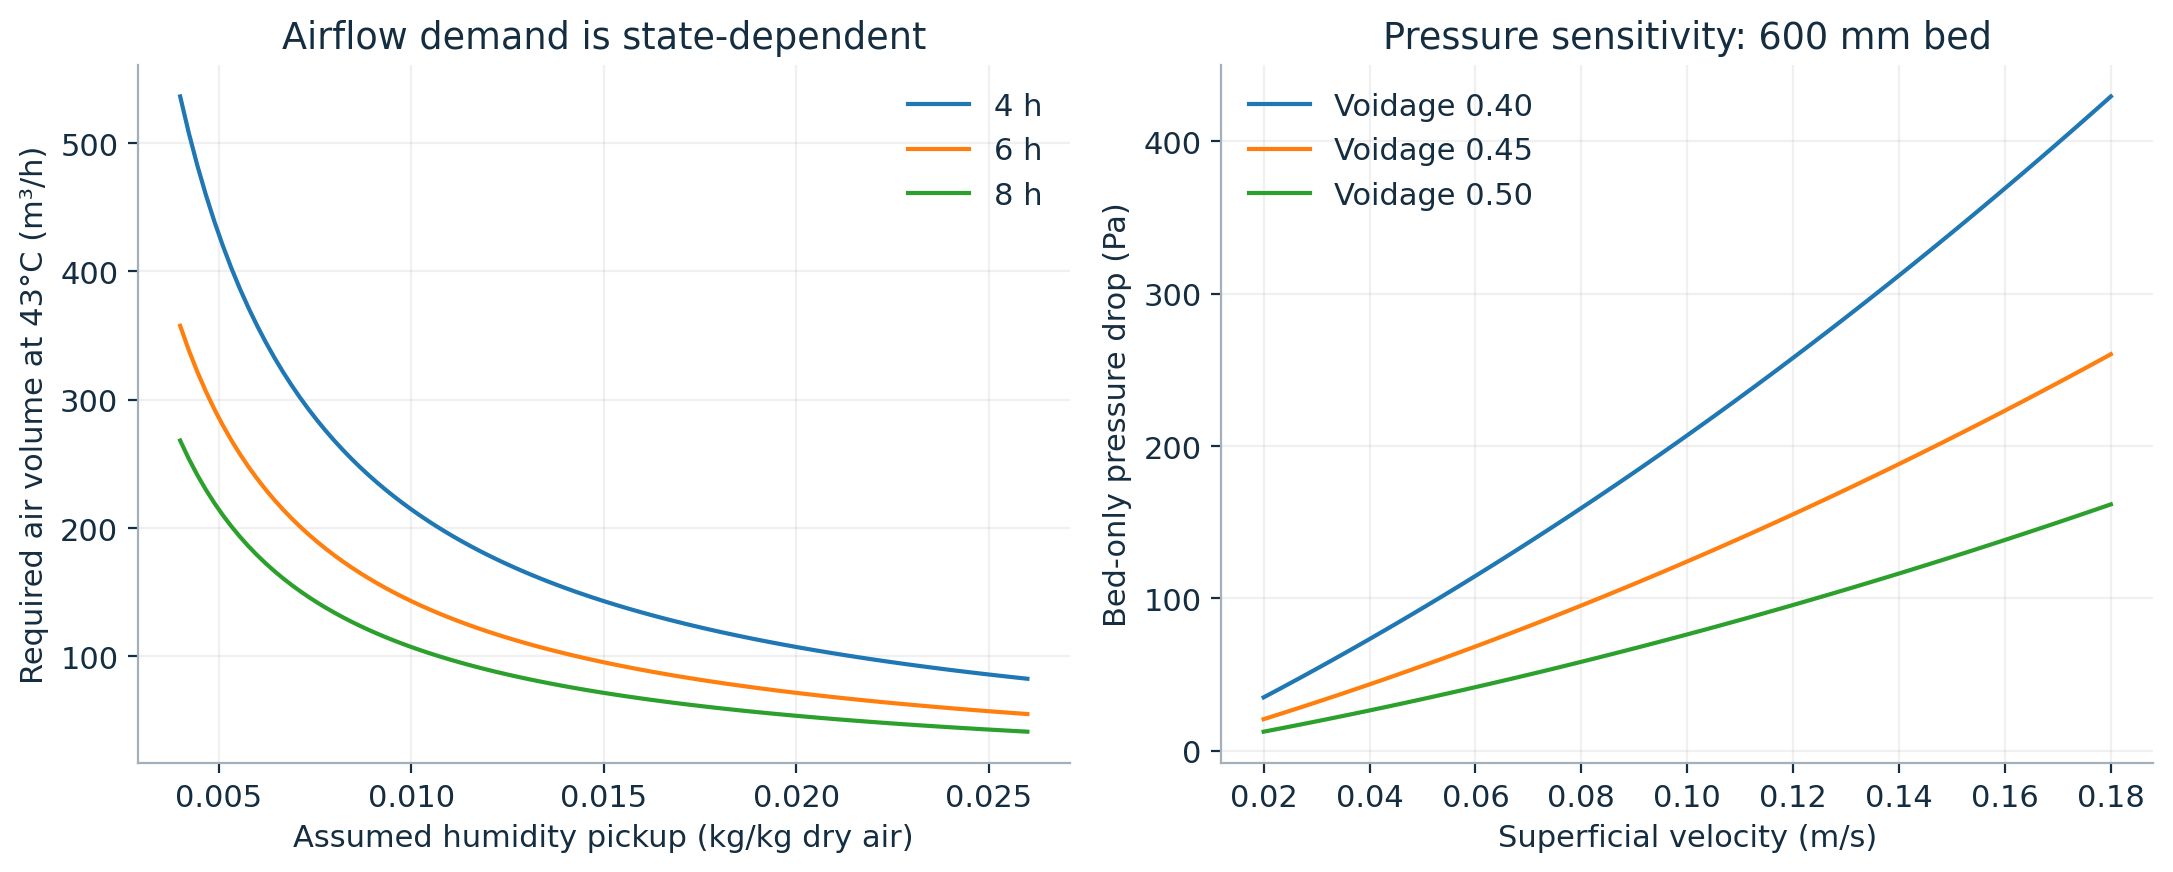
\includegraphics[width=\linewidth]{../figures/sensitivity.png}
\sect{10. Sensitivity and planned measurements}
At 43\,\si{\celsius}, six hours and the same ambient humidity, assume $\Delta\omega$ only as a parameter (not a thermodynamically verified outlet). Increasing pickup from 0.005 to 0.010 halves the algebraic air demand from about 286 to 143 m$^3$/h. A longer time similarly reduces mean demand. Pressure rises with velocity and is sensitive to voidage. Measure calibrated flow and pressure at several settings, plus grain temperatures and MC at 3 heights and 2 radii. Compare $\Delta m$ with $\int \dot m_{da}(\omega_o-\omega_i)dt$. Report specific energy $SEC=E_{input}/m_{ev}$ in kWh/kg removed, and identify whether solar or fuel energy is included. Evaluate moisture spread and rice quality; repeat trials.\par
\textbf{Source trail:} Project reports 9 and 29 October 2026; FAO \href{https://www.fao.org/4/T1838E/T1838E0u.htm}{drying principles}; Ergun (1952) \href{https://www.industrydocuments.ucsf.edu/tid/efk76a99/pdf}{packed columns}; Tohidi et al. (2017) \href{https://doi.org/10.1016/j.rser.2016.11.196}{deep-bed drying}; Anchal et al. (2020) \href{https://doi.org/10.9734/cjast/2020/v39i530546}{thin-layer models}. Numerical calculations reproduced in \texttt{model.py}; this is not a simulation or a drying trial.
\end{document}
